\documentclass[tikz]{standalone}

\usepackage[latin1]{inputenc}
\usepackage{tikz}

% GNUPL
\begin{document}
\pagestyle{empty}


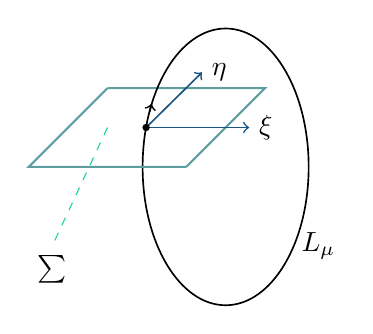
\begin{tikzpicture}
    scale=0.7;
    \draw[color={rgb,255:red,95; green,158; blue,160},thick] (-1,4) -- (1,4) -- (0,3);
    \draw[semithick] (0.5,3) ellipse (30pt and 50pt);
    \draw[color={rgb,255:red,95; green,158; blue,160},thick] (0,3) --(-2,3) -- (-1,4);
    \draw[dashed,color={rgb,255:red,28; green,211; blue,162}] (-1,3.5) -- (-1.7,2);
    \coordinate [label=-90:$\sum$] (8) at (-1.7,2);
    \draw[semithick][->] (-0.465,3.7) -- (-0.44,3.8);
    \draw[semithick, color={rgb,255:red,27; green,85; blue,131}][->] (-0.51,3.5) -- (0.2,4.2);
    \draw[semithick, color={rgb,255:red,27; green,85; blue,131}][->] (-0.51,3.5) -- (0.8,3.5);
    \coordinate [label=0:$\eta$] (8) at (0.2,4.2);
    \coordinate [label=0:$\xi$] (8) at (0.8,3.5);
    \coordinate [label=0:$L_{\mu}$] (8) at (1.34,2);
    \draw[semithick][fill] (-0.51,3.5) ellipse (1pt and 1pt);

\end{tikzpicture}


\end{document}